%%
%% Author: shoupu_wan
%% 7/14/18
%%

\chapter{Recursive programming} \label{ch:recursion}

The concept of recursion has long been known to artists and is present in many distinct
disciplines: linguistics, logic, mathematics.
In computer science, recursion becomes its central idea for developing both data structures and
procedures.
Many recursive data structures, generally falling in the linked data structure category, consist
of the most important applications: linked lists, trees, \textit{etc}.
In this chapter, we are going to discuss the \emph{practical} aspects of
recursion, recursive procedures, and recursive functions.

Recursive function has a close connection with dynamic programming.
Recursive functions are the
Do not think recursions as an infinite loop.
Instead, recursive function execution is a spiral.

Like a sourdough recipe calling for some dough left over from the last time the same recipe was
made.

Like a spiral maze, recursive function execution will
Recursions are a special kind of loop.
Ordinary loop such as \code{for}, \code{while} or \code{do-while} relies on local variables to
control the execution.
Recursion on the other hand relies on stack variables, which include variables you passed in when
recursively calling functions, to control the execution.

The questions when it comes to thinking of the base cases are:
What if the matrix is a row array?
Column array?
What if the matrix is a one-cell matrix?
Extreme question: what if the matrix is empty?
Do you just throw exception?

\begin{figure}[htb]
    \lstinputlisting[label={lst:matrix-spiral-term},
    caption={Matrix spiral print termination position.}]
    {if-else/spiral_termination_position.py}
\end{figure}

\section{Convert Recursive Solutions to Iterative}\label{sec:convertRecursiveSolutionsToIterative}

How to convert recursive solution to iterative?

\section{Base Case Reduction Technique}\label{sec:baseCaseShrinkingTechnique}
Choose a base case that's both small and with an obvious solution.
The choice of a base case contains an aesthetic sense, is reflective to one's
engineering taste, and thus needs some training.

One of the criteria for a good base class is that that it requires minimal initialization.

\section{Taxonomy of recursive functions}\label{sec:taxonomy-recursive-functions}

Functions become recursive because of the occurrence(s) of recursive function invocation.
Depending on the number of recursive function invocations, recursive functions are classified
into single and multiple recursive functions.
The \emph{single recursive function}s are those that make exactly one recursive calls, whereas
\emph{multiple recursive function}s are those that make more than one recursive function
invocations in the function definition.
Note some recursive functions make recursive calls in a loop.
So even though there is only one recursive invocation, these are considered multiple recursive
functions.
One of the main reason for differentiating single and multiple recursive functions
is for time complexity analysis.

Another way for recursive function classification is based on how many participant functions
there are in the recursive calls.
Ordinary recursive functions involve only one function and self invocation(s).
When there are more than one mutually recursive participant functions and hetero-invocations, all
the participating functions will be called \emph{mutually recursive functions}.
Mutual recursions in function design have important application in text parsing and compositional
recursive data processing, \textit{etc.}
We will discuss mutual recursion in later sections of this chapter.
For a real-world example of applications of mutual recursions, see ~\autoref{ch:json-prettifier} in
~\fullref{prt:advanced}.

\section{General design considerations of recursive functions}\label{sec:generalRecursiveFunction}


\section{Remnant function parameter}\label{sec:remnantFunctionParameter}

Some parameters are used only by recursive calls and
client code who invokes this function never need to specify.
So we may dub it as `remnant function parameter'.

One could create a simpler function wrapping around this one to get rid of the remnant
parameter.
As an effort to take the burden away from client code to specify a confusing, useless parameter,
it is given a default value as a clumsy remedy.

\section{Tail Recursion}\label{sec:tailRecursion}

If last action of a function is an invocation of itself, then this recursive function is called a
tail recursive function\footnote{\url{https://en.wikipedia.org/wiki/Tail_call}}.

\section{Recursion and mathematical induction}\label{sec:recursionAndMathematicalInduction}
Mathematical induction\footnote{\url{https://en.wikipedia.org/wiki/Mathematical_induction}}

\section{Mutual recursion}\label{sec:mutual-recursion}

\section{Multivariate recursive functions}\label{sec:multivariateRecursiveFunctions}
\begin{defn}
    A group of multivariate functions are recursive iff the invocation graph is not a directed
    acyclic graph.
\end{defn}

When dealing with a task that is a recursive composition of subtasks of a few
distinct types, multiple mutually recursive functions,
with each function dedicates to solve tasks of one category,
usually make a solution with highly cohesive code.
A beautiful example may be found in the book ~\cite{Beautiful-Code:2007} chapter 1 for the regular
expression \code{grep} function.
For an example in this book, reader can refer the JSON parser of ~\fullref{ch:json-prettifier}.

Topology for multi-function recursion are usually star-shaped---a main function for dispatching,
one or more leaf functions that only interact with the main function.

\begin{figure}[H]
    \centering
    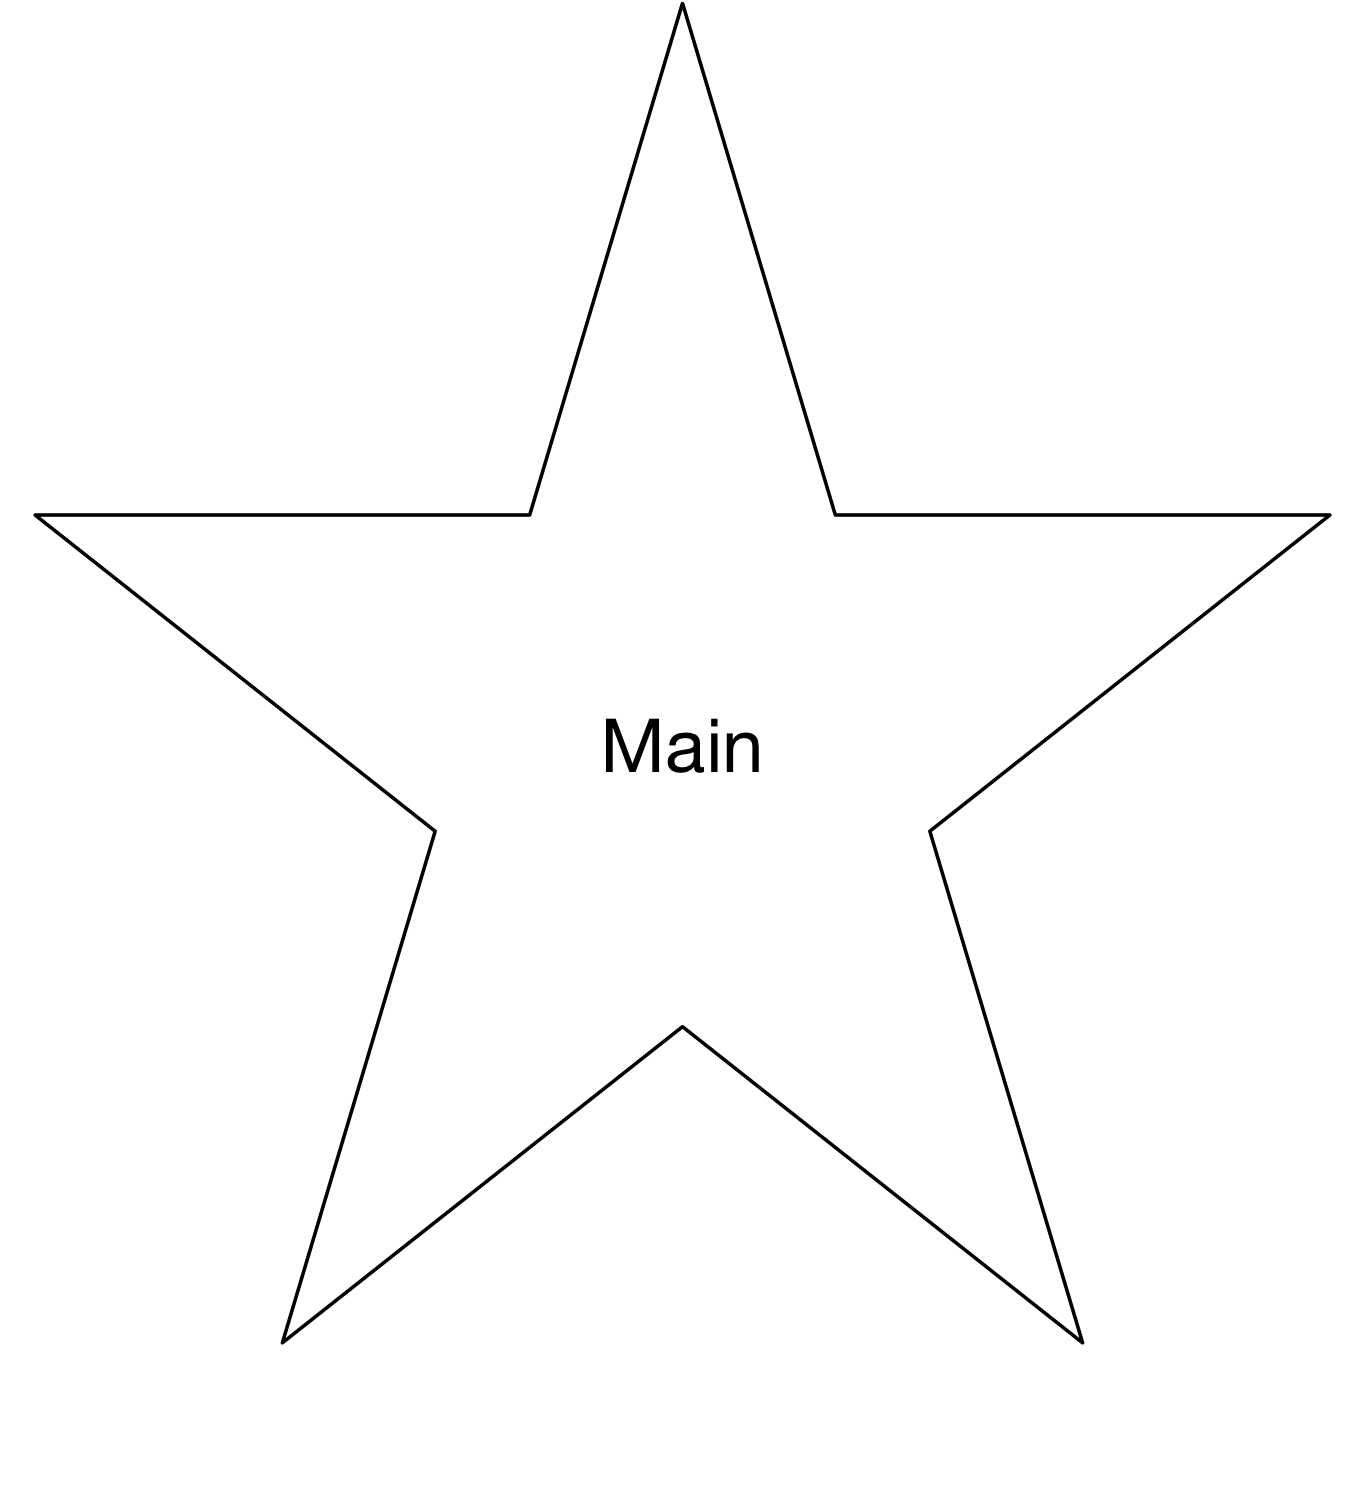
\includegraphics[width=\textwidth]{recursion/multi-recursion.jpg}
    \caption{Asymmetric cycle division.\label{fig:cycle.division.asymmetric}}
\end{figure}

Each function in the mutual recursion group
implementation has its specialty and is the sole expert for performing a duty.
No function should perform this specialty except the designated function.
When other functions need to perform this duty, they have to defer it to the designated function.

\section{Stumbling block in recursion}\label{sec:stumblingBlockInRecursion}

Stack is a state machine for recursion.
Make sure that your other stateful variables do not interfere with this.
One technique to reduce risk of modifying state of variables is to use immutable variables such
as \code{string}, \code{tuple}, \code{pair}, \textit{etc.}

The following code snippet suffers this problem.
\lstinputlisting{recursion/bad-recursion.py}
